%% Intrapartum standard-plane classification: a negative-results study.
%% IEEE conference format (IEEEtran). Build instructions: paper/README.md
\documentclass[conference]{IEEEtran}

\usepackage{cite}
\usepackage{amsmath,amssymb}
\usepackage{graphicx}
\usepackage{booktabs}
\usepackage{url}
\usepackage[hidelinks]{hyperref}

\begin{document}

\title{What Survives Three Seeds: A Negative-Results Study of\\
Frame Sampling, Segmentation and Shortcut Learning in\\
Intrapartum Ultrasound Standard-Plane Classification}

\author{\IEEEauthorblockN{M.~V.~S.~Akhil Teja}
\IEEEauthorblockA{\textit{Independent researcher}\\
\url{github.com/AkhilTeja2209/intrapartum-plane-density}}}

\maketitle

\begin{abstract}
Automatic detection of standard planes in intrapartum transperineal ultrasound
is usually reported as a single accuracy figure from a single training run. We
argue that this practice is inadequate for corpora of this size, and support
the argument with a study in which most reported effects dissolve under
replication. On the IUGC~2024 corpus (774 videos, 65{,}531 frames) we run 25
classifier arms and 21 U-Net arms, and measure every difference against a
three-seed spread. Three findings follow. First, a controlled frame-sampling
study is inconclusive by construction: the budget-matched comparison reverses
sign across seeds and one condition moves 0.231 macro-F1 on identical data,
exceeding every density effect. Second, of five segmentation design choices
re-run at three seeds, only one survives---feeding the network frames decoded
at the masks' native resolution ($+0.0163$ Dice, $t=3.79$)---while a ResNet-34
encoder reverses sign between one seed and three, and removing augmentation
leaves the mean unresolved but triples the seed spread. Third, and most
consequential, the test set contains two acquisition campaigns three years
apart, and no model transfers between them: the gap in AUROC is positive in 25
of 25 arms (mean $+0.179$), and the best-scoring model overall is at chance on
the older campaign (AUROC 0.579, 95\% CI [0.495, 0.667]). That model is also
the one a Grad-CAM analysis shows attends least to the anatomy (1.12/1.04
against 1.96/1.47 for a frame-wise baseline), giving two independent
instruments the same answer. We report two claims from our own earlier drafts
that did not survive, release every arm's predictions, and deploy both stages
as a browser demo in which each displayed number is checked against a PyTorch
reference at run time.
\end{abstract}

\begin{IEEEkeywords}
medical image analysis, obstetric ultrasound, standard plane detection,
semantic segmentation, distribution shift, shortcut learning, reproducibility,
negative results
\end{IEEEkeywords}

\section{Introduction}

The angle of progression, measured between the pubic symphysis and the fetal
head on a transperineal ultrasound frame, is a quantitative marker of labour
progress. The measurement is valid only on a \emph{standard plane}: a frame in
which both structures are resolved well enough to be delineated. Automating the
selection of such frames is therefore a prerequisite for automating the
measurement, and it is the task addressed here.

The literature on this task, as on much of medical imaging, reports
single-number results: one architecture, one training run, one test score. Our
central claim is methodological. On a corpus of a few hundred videos, the
seed-to-seed variation of an ordinary training pipeline is large enough to
manufacture most of the effects such studies report. We demonstrate this not in
the abstract but on our own work: we state what we first measured, what we
concluded, and what happened to those conclusions when each arm was replicated.

Our contributions are:

\begin{enumerate}
\item A controlled frame-sampling study, built so that sparse and dense regimes
differ only in frames drawn per video, which we report as \textbf{inconclusive}
because its seed variance exceeds its effect size (Sec.~\ref{sec:sampling}).
\item A 21-arm segmentation sweep in which each candidate within $2\sigma$ of
baseline was re-run at three seeds. One effect survives; two single-seed
results are withdrawn, one having reversed sign (Sec.~\ref{sec:seg}).
\item An attention analysis extended to negative frames using the segmenter's
predicted masks, validated at $r\approx0.93$ against ground truth where both
exist (Sec.~\ref{sec:attention}).
\item Identification of two acquisition campaigns in the test split, and the
finding that no model transfers between them, in 25 of 25 arms
(Sec.~\ref{sec:campaign}). To our knowledge this is not reported for this
corpus.
\item A browser deployment in which both stages run client-side and every
number is verified against PyTorch at run time; obtaining it required
reproducing Pillow's fixed-point resampling arithmetic exactly
(Sec.~\ref{sec:deploy}).
\end{enumerate}

\section{Data}
\label{sec:data}

We use the IUGC~2024 intrapartum ultrasound dataset (Zenodo
10.5281/zenodo.17655183, CC-BY-4.0): 774 videos and 65{,}531 extracted frames,
with the official splits used unchanged (Table~\ref{tab:data}). A subset of
2{,}915 frames across 606 videos carries pixel-level masks of the pubic
symphysis (PS) and fetal head (FH); every masked frame is a standard plane.

\begin{table}[t]
\caption{Corpus and official splits, used unchanged.}
\label{tab:data}
\centering
\begin{tabular}{lrrr}
\toprule
Split & Videos & Frames & Prevalence \\
\midrule
Train & 434 & 53{,}996 & 0.418 \\
Validation & 40 & 2{,}870 & 0.556 \\
Test & 300 & 8{,}665 & 0.556 \\
\midrule
Total & 774 & 65{,}531 & \\
\bottomrule
\end{tabular}
\end{table}

\subsection{Three acquisition campaigns}
\label{sec:campaigns-data}

The filenames encode acquisition dates in three mutually exclusive
conventions, and these align \emph{exactly} with the official splits:

\begin{itemize}
\item \textbf{Train}: 434 videos, \texttt{20190726T095643\_0} style,
Jul 2019--Jan 2020.
\item \textbf{Test-A}: 93 videos, \texttt{202012132137152159400I1} style,
Dec 2020--Jul 2021.
\item \textbf{Test-B}: 207 videos, \texttt{240422145736} style, Apr--Jul 2024.
\item \textbf{Validation}: 40 videos, renamed to \texttt{test\_10\_80} style;
provenance unrecoverable.
\end{itemize}

Two consequences follow. Every result on this corpus is already measured under
a 1.5-to-4.5-year acquisition shift, a stronger generalisation setting than a
random split. And the test set is internally heterogeneous, which
Sec.~\ref{sec:campaign} exploits.

A per-centre split, which would separate ``reads anatomy'' from ``reads this
hospital's scanner'' directly, is \emph{not possible} on this release: it
carries no centre or hospital field, and all 774 videos are re-encoded to an
identical $512\times512$, 24\,fps, single-codec container, so no device
signature survives in metadata either. The training split is also a single
campaign, leaving nothing to hold out.

\subsection{A small label shortcut}

About 1.3\% of test frames are essentially blank---mean 8-bit luminance below
5, the probe off the body or a transition---and in a 1{,}500-frame sample all
20 such frames are labelled non-standard, without exception. This makes roughly
2.9\% of the negative class available to any model that learns ``black,
therefore not a standard plane,'' requiring no anatomy. It is too small to
explain the effects below and points the wrong way for Sec.~\ref{sec:campaign},
but it is the kind of free lunch that should be subtracted from a headline
number before the number is believed.

\section{Frame sampling density}
\label{sec:sampling}

\subsection{Design}

Sparse (``image dataset'') and dense (``video dataset'') regimes are
constructed from one corpus by varying only the frames drawn per video:
$k\in\{1,2,5,10,20\}$ frames per video for sparse arms, strided and all-frame
arms for dense ones. Because dense arms see more frames in total, we add
\emph{budget-matched} arms (equal total frames) and \emph{prior-matched} arms
(equal class prior), separating density from sample count and from class
balance.

\subsection{Result: inconclusive, and why that is the finding}

Table~\ref{tab:sampling} gives the conditions run at three seeds. The headline
numbers suggest sparse sampling wins. The seed spreads say otherwise.

\begin{table}[t]
\caption{Frame-sampling conditions at three seeds, test macro-F1. Spread,
not mean, is the operative column.}
\label{tab:sampling}
\centering
\begin{tabular}{lrrr}
\toprule
Condition & Mean & SD & Range \\
\midrule
\texttt{sparse\_k1} & 0.6823 & 0.0529 & 0.627--0.733 \\
\texttt{sparse\_k5} & 0.6383 & 0.0503 & 0.586--0.686 \\
\texttt{dense\_all} & 0.6102 & 0.0315 & 0.579--0.642 \\
\texttt{dense\_prior\_matched\_k5} & 0.6076 & \textbf{0.1193} & 0.475--0.707 \\
\texttt{dense\_matched\_k5} & 0.5764 & 0.0343 & 0.537--0.599 \\
\bottomrule
\end{tabular}
\end{table}

The budget-matched comparison---the one designed to isolate density---gives
$-0.106$, $+0.013$ and $-0.093$ across three seeds: it \emph{reverses sign}.
One condition, \texttt{dense\_prior\_matched\_k5}, spans 0.231 macro-F1 on
identical data with only the seed changed. No density effect in this study
exceeds that.

We therefore report the sampling study as inconclusive. This is not a failure
of the design, which we believe sound; it is a measurement of how much signal a
corpus of 434 training videos can support. A single-seed version of this same
experiment would have yielded a publishable-looking density effect in either
direction, depending only on the seed drawn.

\subsection{The temporal arm, and what it is not}

A CNN-BiLSTM over clips reaches 0.670 macro-F1 against 0.579 for the frame-wise
model on the same \texttt{dense\_all} condition. The natural reading is that
temporal context helps. An ablation removing transition splicing---the
mechanism by which the temporal arm is supposed to learn plane entry and
exit---still reaches 0.650, retaining most of the gain. Whatever the temporal
arm is doing, it is largely not transition modelling.
Sections~\ref{sec:attention} and~\ref{sec:campaign} give two further and
independent reasons to doubt the interpretation.

\section{Segmentation}
\label{sec:seg}

\subsection{An evaluation-protocol correction}

Masks and source videos are both $512\times512$, but the frame cache stores a
256-pixel short side. An arm nominally trained at 384\,px is therefore fed
interpolated pixels, and scoring it at its own input size compares against a
downsampled mask. We re-score every arm one way: predictions resampled back to
$512\times512$ and compared against untouched ground truth, the protocol the
published 0.893--0.930 range for this corpus uses. Re-scoring our original run
this way moves it from 0.8699 to 0.8661---the earlier figure was optimistic by
0.004 purely through the evaluation grid.

\subsection{Three seeds per contested arm}

The baseline spread over three seeds is $0.8665\pm0.0034$. Every arm whose
single-seed result sat within about $2\sigma$ of it was re-run at seeds 1 and 2
(Table~\ref{tab:seg}).

\begin{table}[t]
\caption{Segmentation arms at three seeds. Baseline $0.8665\pm0.0034$
(mean foreground Dice, native $512^2$ scoring).}
\label{tab:seg}
\centering
\small
\setlength{\tabcolsep}{4pt}
\begin{tabular}{lrrrrl}
\toprule
Arm & Mean & SD & $\Delta$ & $t$ & Verdict \\
\midrule
\texttt{native384} & 0.8828 & 0.0066 & $+0.0163$ & $+3.79$ & \textbf{resolved} \\
\texttt{native256} & 0.8695 & 0.0040 & $+0.0030$ & $+0.97$ & unresolved \\
\texttt{resnet34} & 0.8673 & 0.0052 & $+0.0008$ & $+0.22$ & unresolved \\
\texttt{noaug} & 0.8571 & 0.0106 & $-0.0094$ & $-1.46$ & unresolved \\
\texttt{size384} (cached) & 0.8567 & 0.0178 & $-0.0098$ & $-0.94$ & unresolved \\
\bottomrule
\end{tabular}
\end{table}

\textbf{One effect survives.} Feeding the network frames re-decoded at the
masks' native resolution, at 384\,px, is worth $+0.0163$ Dice at $t=3.79$. It
is a data-handling fix, not an architectural one.

\textbf{Two single-seed results do not.} A ResNet-34 encoder read as $-0.0052$
at one seed and is $+0.0008$ at three: the sign reversed, and our earlier
statement that ``more encoder is the wrong direction at this sample size'' is
withdrawn---it is no direction at all. The \texttt{native256} effect halved,
from $+0.0066$ to $+0.0030$, so native decoding is not itself the win; 384\,px
is.

\textbf{Resolution is not the whole story.} Native 384\,px gains $+0.0163$ with
SD 0.0066, whereas \emph{cached} 384\,px---the same input size, interpolated up
from the 256\,px cache---loses 0.0098 with SD 0.0178, five times the baseline
spread, its worst seed scoring 0.8361. Requesting a resolution the pixels do
not contain is worse than not requesting it, and it destabilises training.

\textbf{Variance can be the effect.} Removing augmentation does not resolve as
a mean shift ($t=-1.46$) but triples the seed spread (0.0106 against 0.0044).
On this corpus augmentation buys stability rather than expected Dice---a
statement a single-seed experiment cannot make at all.

The best single arm is \texttt{native384\_s1} at 0.8897; averaging the shipped
configuration over its own three seeds reaches \textbf{0.8913}, against 0.8859
for averaging three different input resolutions. The apparent benefit of
``resolution diversity'' in ensembling was seed-averaging throughout.

\subsection{The validation split ranks almost at random}

Over 21 arms, validation and test Dice correlate at Pearson $r=+0.42$,
Spearman $\rho=+0.28$. At that rank correlation, ``best on validation'' carries
almost no information. With the three \texttt{native384} seeds present the
validation argmax happens to coincide with the test argmax, so selection costs
0.0 Dice; over the earlier 11 arms it cost 0.0187. \emph{Neither number is a
property of the split.} A selector with $\rho=0.28$ that lands on the best of
21 arms has been lucky. What is stable across both passes is the correlation,
and it is poor. Forty validation masks from 40 videos are not enough to rank
models on this task.

\subsection{A withdrawn claim: the segmenter as a classifier}
\label{sec:derived}

A segmenter trained only on standard planes can be turned into a classifier by
thresholding how much anatomy it finds. Our first result reported 0.607
macro-F1 for this rule against 0.610 for the dense frame classifier, and called
it a match. Across eleven arms the rule gives $0.530\pm0.039$, well below the
frame classifier's $0.610\pm0.032$: the original figure was one seed at the top
of a wide distribution.

A weakened version---``the best configurations do reach the frame
classifier''---also failed. It rested on \texttt{native384\_s0} scoring 0.603.
The same configuration at seed~1, which has the best Dice in the entire sweep,
scores \textbf{0.456} (Table~\ref{tab:derived}): 0.147 lower, and below every
baseline seed. Better segmentation does not buy a better derived classifier,
and ``best'' is identifiable only after the fact.

\begin{table}[t]
\caption{Area-derived classifier. The rule is selected on validation per arm;
test macro-F1 does not follow it.}
\label{tab:derived}
\centering
\begin{tabular}{llrrr}
\toprule
Arm & Rule & Val F1 & Test F1 & Specificity \\
\midrule
\texttt{base\_s0} & geomean & 0.603 & 0.577 & 0.245 \\
\texttt{base\_s1} & sum & 0.573 & 0.494 & 0.143 \\
\texttt{base\_s2} & geomean & 0.640 & 0.498 & 0.144 \\
\texttt{ens\_seeds} & geomean & 0.587 & 0.587 & 0.260 \\
\texttt{native384\_s1} & geomean & 0.565 & \textbf{0.456} & 0.099 \\
\bottomrule
\end{tabular}
\end{table}

Threshold-free AUPRC is far more stable at $0.757\pm0.024$. What is unreliable
is converting a segmented area into a decision, not the segmenter's ordering of
frames. The error profile is the substance: the shipped arm runs at recall
0.993 against specificity 0.099, calling 90\% of non-standard frames standard.
It is not a plane detector; it is an anatomy detector asked a question it was
never supervised for, and sharpening its segmentation makes it \emph{more}
confident on frames containing anatomy but no standard plane.

\section{Where the classifiers look}
\label{sec:attention}

\subsection{Method}

We compute Grad-CAM over the classifier's prediction and measure the fraction
of total activation falling inside the PS$+$FH mask, divided by what an
equal-area random region would collect. A ratio near 1.0 means the model is not
using the anatomy: it is reading depth markers, UI overlay, the sector fan or
speckle statistics.

Ground-truth masks exist only for standard planes, so this check could
originally be run only on positives---which leaves open exactly the possibility
of interest, that a model attends to anatomy when anatomy is present and to
scanner furniture when it is not. We close this by having the U-Net predict
masks for every frame including negatives. Predicted and ground-truth masks
agree at $r\approx0.93$ on frames that have both, which is the evidence for
using predicted masks alone elsewhere.

\subsection{Result}

\begin{table}[t]
\caption{Anatomical attention ratio by class, predicted masks, 120 frames per
class. $n$ is frames yielding a usable ratio.}
\label{tab:attention}
\centering
\begin{tabular}{lrrr}
\toprule
Model & macro-F1 & Standard ($n$) & Non-std.\ ($n$) \\
\midrule
ResNet-18 \texttt{dense\_all} & 0.579 & \textbf{1.96} (120) & 1.47 (118) \\
ResNet-18 \texttt{sparse\_k1} & 0.687 & \textbf{1.88} (120) & 1.51 (114) \\
CNN-BiLSTM, no splice & 0.650 & 1.20 (113) & 1.45 (89) \\
CNN-BiLSTM, spliced & 0.670 & \textbf{1.12} (120) & \textbf{1.04} (93) \\
\bottomrule
\end{tabular}
\end{table}

Frame-wise models read anatomy on both classes; temporal models largely do not
(Table~\ref{tab:attention}). The best-scoring model attends to the anatomy
least, on both classes, and splicing makes attention \emph{worse}---a second
line of evidence, independent of the ablation in Sec.~\ref{sec:sampling}, that
the temporal arm's advantage is not better frame understanding.

Two counts deserve reporting alongside. The segmenter drew anatomy on
\emph{every} frame of all four runs, including all 120 non-standard ones, which
is the over-calling of Sec.~\ref{sec:derived} observed directly. And the
temporal models produce an all-zero Grad-CAM---no positive evidence
anywhere---on 27 and 31 of 120 negatives, against 2 and 6 for the frame models.
Those frames yield no ratio, so the non-standard means are computed with the
most confidently negative frames excluded. We report the counts rather than
silently shrinking the denominator.

\section{Cross-campaign transfer}
\label{sec:campaign}

Since a per-centre split is impossible (Sec.~\ref{sec:campaigns-data}), we
score the two test campaigns separately. This asks the same question from
predictions that already exist, with no retraining.

\subsection{Protocol}

We report AUROC. The campaigns differ in prevalence (0.683 against 0.521), so
neither macro-F1 at one frozen threshold nor AUPRC---whose baseline \emph{is}
the prevalence---can be read across them. Intervals resample
\emph{examinations}, not clips: the 2021 filenames encode an examination stamp
followed by \texttt{I1}--\texttt{I6}, so its 93 clips are 33 examinations, and
the 2024 clips, a median of 1.3 minutes apart, group into 84 sessions under a
10-minute rule. Resampling clips treats correlated units as independent and
reports intervals that are too narrow.

\subsection{Result}

\begin{table}[t]
\caption{Per-campaign AUROC. Intervals resample examinations (33 and 84 units
respectively).}
\label{tab:campaign}
\centering
\small
\begin{tabular}{lrrr}
\toprule
Model & 2021 & 2024 & Gap [95\% CI] \\
\midrule
\texttt{sparse\_k1} & 0.699 & 0.861 & $+0.162$ [0.079, 0.252] \\
\texttt{dense\_all} & 0.630 & 0.813 & $+0.183$ [0.098, 0.267] \\
BiLSTM, spliced & \textbf{0.579} & 0.844 & $+0.266$ [0.177, 0.357] \\
BiLSTM, no splice & 0.592 & 0.787 & $+0.195$ [0.103, 0.294] \\
\bottomrule
\end{tabular}
\end{table}

No model transfers (Table~\ref{tab:campaign}). All four gaps exclude zero, and
this is not a thresholding artifact: re-tuning the threshold per campaign---on
test, as a diagnostic---still leaves 2021 at 0.57--0.65 macro-F1 against
0.72--0.80 on 2024. Ranking degrades, not merely calibration.

\textbf{The effect is unanimous.} Across all 25 arms with saved
predictions---every sampling condition, seed and architecture---mean AUROC is
0.632 on 2021 against 0.810 on 2024. The gap is positive in \textbf{25 of 25}
arms (mean $+0.179$, median $+0.184$, range $+0.047$ to $+0.299$), and 9 of 25
fall below 0.60 on 2021. The best 2021 result anywhere in the study is 0.770. A
unanimous sign is a property of the shift, not of any model.

\textbf{The best model fails worst.} The spliced CNN-BiLSTM leads overall at
0.670 macro-F1 and collapses hardest: AUROC 0.579, with an interval of
[0.495, 0.667] that \emph{includes} 0.5. On 33 examinations it is
statistically indistinguishable from a coin flip. This agrees with
Sec.~\ref{sec:attention} from the opposite direction---least anatomical
attention, worst transfer.

\textbf{It is not temporal drift.} Training is 2019, so 2021 is the campaign
\emph{nearer} in time, and it is the one that fails, by 0.18 AUROC on average.
Elapsed time since training does not explain this, which is what makes some
property of the 2021 acquisition setup the more plausible reading.

Why the headline numbers look healthy: 2024 contributes 207 of 300 test videos,
so aggregate figures are dominated by the campaign every model handles well.

\section{Browser deployment}
\label{sec:deploy}

Both stages run client-side via onnxruntime-web; no image leaves the device
(Fig.~\ref{fig:demo}). The classifier is 44.7\,MB and the U-Net 57.3\,MB,
fetched on demand. Dynamic int8 quantisation reduces the segmenter to 14.4\,MB
at no measurable Dice cost, but onnxruntime-web provides no
\texttt{ConvInteger} kernel, so the fp32 graph ships.

\begin{figure}[t]
\centering
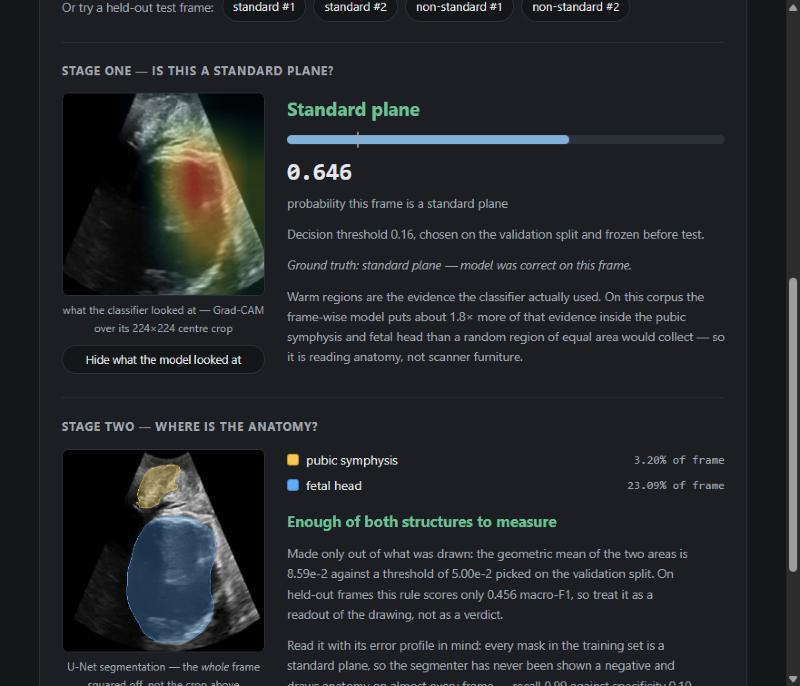
\includegraphics[width=\columnwidth]{../docs/demo.png}
\caption{Both stages on a held-out standard plane. Stage one scores the frame
and shows Grad-CAM evidence over its $224^2$ crop; stage two outlines the
symphysis and head on the whole frame. Each displayed value is checked against
a PyTorch reference in the browser.}
\label{fig:demo}
\end{figure}

Agreement with PyTorch required reproducing Pillow's resampling exactly.
Pillow does not accumulate 8-bit bilinear resampling in floating point: it
quantises filter weights to 22-bit fixed point and shifts back. On the
$256\rightarrow384$ upscale the segmenter needs, a third of output pixels land
on exact half-way blends, and the two roundings disagree on \textbf{14.5\% of
pixels}. Porting the fixed-point path reproduces Pillow on all 147{,}456 pixels
and takes browser-versus-PyTorch agreement from $2.6\times10^{-3}$ to
$1.1\times10^{-7}$. A downscale masks the discrepancy, which is why the
classifier path appeared correct while the segmentation path was not.

We regard run-time verification as a reporting practice worth adopting: the
page recomputes the reference comparison on every inference and displays the
result, so a reader need not trust that the deployment matches the reported
model.

\section{Limitations}

The attention analysis on negatives measures agreement with a \emph{predicted}
mask from a segmenter that has never seen a negative and over-calls them, so
the non-standard column answers a weaker question than the standard column; the
$r\approx0.93$ validation covers positives only, as that is where ground truth
exists.

The cross-campaign result establishes that performance does not transfer; it
does not isolate the scanner as the cause. The campaigns are three years apart
and may differ in patient population, operator and protocol as well as
equipment, and no per-centre split exists to separate these. What raises the
shortcut reading above speculation is the correlation with attention: the arm
with the least anatomical grounding degrades most. The 2024 session grouping is
a 10-minute heuristic rather than a stated fact, though since 2024 is the tight
side of every interval, a coarser truth would widen the gaps away from zero.

The 40 validation videos are renamed and cannot be placed in either campaign,
so both model selection and threshold selection rest on 40 videos of unknown
provenance. Finally, \texttt{native512} remains at one seed: at 4.7 hours per
seed for an arm sitting $0.4\sigma$ from baseline, two further seeds were
judged a poor use of compute.

\section{Conclusion}

Across two tasks and 46 training arms on this corpus, the effects that survive
replication are a data-handling fix (native-resolution input, $+0.0163$ Dice)
and two unfashionable recipe choices (the Dice loss term, ImageNet
pre-training). The effects that did not survive include a frame-sampling
density result, an encoder-capacity result that reversed sign, and two
successive versions of a claim that a segmenter can classify.

The finding we consider most important is one no single-split evaluation could
have produced: the test set holds two acquisition campaigns, and no model
transfers between them, in 25 of 25 arms. The model that scores best overall is
at chance on the older campaign, and is independently the model that attends
least to the anatomy. On corpora of this size we recommend reporting a seed
spread before any effect, partitioning the test set by acquisition metadata
wherever filenames permit, and treating a single-split number as a hypothesis
rather than a result.

\section*{Reproducibility}

Code, every arm's test predictions, the full comparison tables and the deployed
demo are at
\url{https://github.com/AkhilTeja2209/intrapartum-plane-density}. The
per-campaign analysis runs from saved predictions without a GPU
(\texttt{python -m tools.per\_campaign}). A synthetic end-to-end smoke test
covering both stages runs in continuous integration.

\section*{Ethical Statement}

This is a research artefact, not a diagnostic tool, and is not validated for
clinical use. It was trained only on third-trimester transperineal video and
returns a confident number for any image, including images unlike its training
data. The dataset is public and used under CC-BY-4.0.

\begin{thebibliography}{9}
\bibitem{iugc2024}
IUGC 2024 Challenge, ``Intrapartum ultrasound grand challenge dataset,''
Zenodo, 2024, doi:10.5281/zenodo.17655183.
\bibitem{unet}
O.~Ronneberger, P.~Fischer, and T.~Brox, ``U-Net: convolutional networks for
biomedical image segmentation,'' in \emph{Proc. MICCAI}, 2015, pp.~234--241.
\bibitem{resnet}
K.~He, X.~Zhang, S.~Ren, and J.~Sun, ``Deep residual learning for image
recognition,'' in \emph{Proc. CVPR}, 2016, pp.~770--778.
\bibitem{gradcam}
R.~R.~Selvaraju \emph{et al.}, ``Grad-CAM: visual explanations from deep
networks via gradient-based localization,'' in \emph{Proc. ICCV}, 2017,
pp.~618--626.
\bibitem{shortcut}
R.~Geirhos \emph{et al.}, ``Shortcut learning in deep neural networks,''
\emph{Nature Machine Intelligence}, vol.~2, pp.~665--673, 2020.
\bibitem{aop}
T.~Ghi \emph{et al.}, ``ISUOG practice guidelines: intrapartum ultrasound,''
\emph{Ultrasound in Obstetrics \& Gynecology}, vol.~52, no.~1, pp.~128--139,
2018.
\end{thebibliography}

\end{document}
